\documentclass[11pt,a4paper]{article}

% Required Packages
\usepackage[utf8]{inputenc}
\usepackage[T1]{fontenc}
\usepackage{lmodern}
\usepackage[margin=1in]{geometry}
\usepackage{amsmath,amssymb,amsthm}
\usepackage{graphicx}
\usepackage{booktabs}
\usepackage{hyperref}
\usepackage{xcolor}
\usepackage{float}
\usepackage{subcaption}
\usepackage{enumitem}
\usepackage{fancyhdr}
\usepackage{tikz}
\usetikzlibrary{shapes,arrows,positioning,calc}

% Algorithm environment
\newfloat{algorithm}{htbp}{loa}
\floatname{algorithm}{Algorithm}

% Colors
\definecolor{accentblue}{RGB}{0,82,147}
\definecolor{codegreen}{rgb}{0,0.6,0}

% Hyperref setup
\hypersetup{
    colorlinks=true,
    linkcolor=accentblue,
    urlcolor=accentblue,
    citecolor=accentblue
}

% Header/Footer
\pagestyle{fancy}
\fancyhf{}
\setlength{\headheight}{14pt}
\fancyhead[L]{Depth Densification Report}
\fancyfoot[C]{\thepage}
\renewcommand{\headrulewidth}{0.4pt}
\renewcommand{\footrulewidth}{0.4pt}

% Title
\title{
    \vspace{-1cm}
    \textbf{Depth Densification from Posed Multi-Camera UAV Images}\\
    \large Technical Report
}
\author{Alibek Erkabayev\\Senior Computer Vision Engineer}
\date{March 2026}

\begin{document}

% Title page
\begin{titlepage}
\centering
\vspace*{3cm}
{\LARGE\bfseries Depth Densification from Posed\\Multi-Camera UAV Images\par}
\vspace{0.5cm}
{\large Technical Report\par}
\vspace{2cm}
{\Large Alibek Erkabayev\par}
\vspace{0.3cm}
{\large Senior Computer Vision Engineer\par}
\vspace{3cm}
{\large March 2026\par}
\vfill
\end{titlepage}

%==============================================================================
\begin{abstract}
\noindent
This report presents a depth densification pipeline for UAV imagery captured by a multi-camera system with nadir and oblique views. The pipeline combines Structure-from-Motion (COLMAP) for sparse 3D reconstruction with monocular depth estimation (Depth Anything V2) to produce dense depth maps. A polynomial regression model using Ordinary Least Squares (OLS) maps the relative inverse-depth predictions to depth in the SfM scale using sparse 3D anchor points. On a 90-image multi-view UAV survey set (nadir and oblique views), the average Mean Absolute Error (MAE) is 0.19\,m and the Root Mean Square Error (RMSE) is 0.35\,m. These errors are residuals at the SfM anchor points used for the fit (in-sample), not a held-out evaluation, and the depth is expressed in the scale of the SfM reconstruction (Section~\ref{sec:limits}).
\end{abstract}

%==============================================================================
\section{Introduction}
%==============================================================================

The goal is to produce dense depth maps from multi-camera UAV imagery. The survey set used for the reported numbers is a 90-image multi-view UAV survey with nadir and oblique views.

The pipeline has four stages:
\begin{itemize}[noitemsep]
    \item \textbf{Stage 1}: Structure-from-Motion (SfM) reconstruction to obtain sparse 3D points and camera poses
    \item \textbf{Stage 2}: Monocular depth estimation to generate dense relative inverse-depth maps
    \item \textbf{Stage 3}: Depth densification via polynomial regression to map relative inverse depth to depth in the SfM scale
    \item \textbf{Stage 4}: C++ implementation of stage 3 with unit tests
\end{itemize}

This report focuses on stage 3: the derivation of the Ordinary Least Squares (OLS) solution, quantitative results, and a discussion of numerical stability, robustness, model selection and failure modes.

%==============================================================================
\section{Pipeline Overview}
%==============================================================================

\begin{figure}[h]
\centering
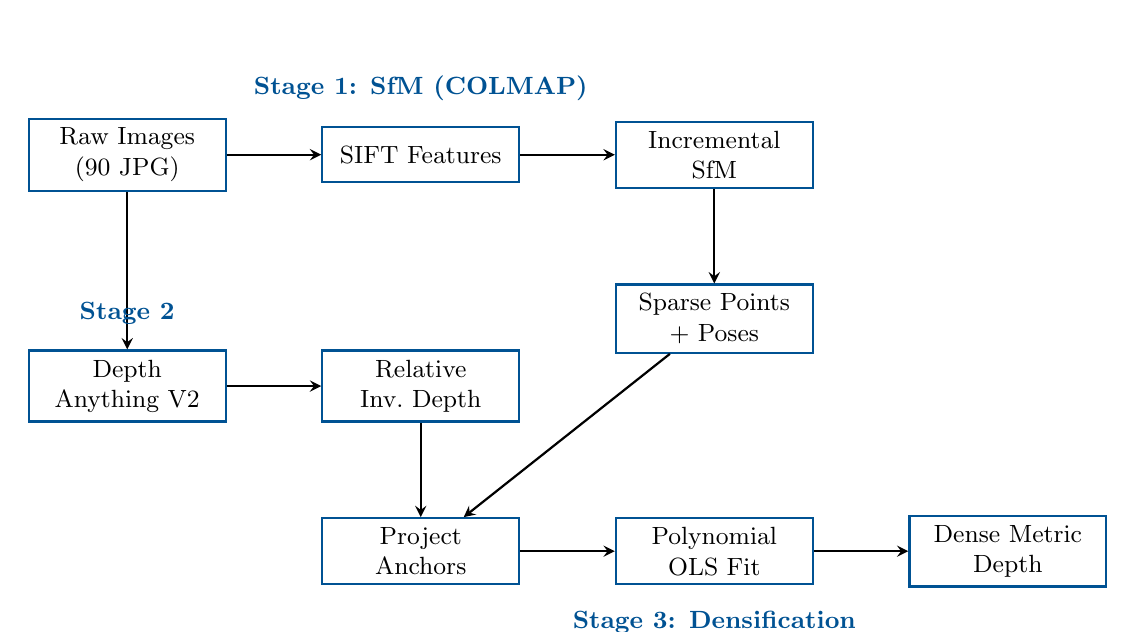
\begin{tikzpicture}[
    node distance=1.2cm,
    box/.style={rectangle, draw=accentblue, thick, minimum width=2.5cm, minimum height=0.7cm, align=center, font=\small},
    arrow/.style={->, >=stealth, thick}
]
    % Stage 1
    \node[box] (images) {Raw Images\\(90 JPG)};
    \node[box, right=of images] (sift) {SIFT Features};
    \node[box, right=of sift] (sfm) {Incremental\\SfM};
    \node[box, below=of sfm] (sparse) {Sparse Points\\+ Poses};

    % Stage 2
    \node[box, below=2cm of images] (mono) {Depth\\Anything V2};
    \node[box, right=of mono] (reldepth) {Relative\\Inv.\ Depth};

    % Stage 3
    \node[box, below=of reldepth] (project) {Project\\Anchors};
    \node[box, right=of project] (ols) {Polynomial\\OLS Fit};
    \node[box, right=of ols] (dense) {Dense Metric\\Depth};

    % Arrows
    \draw[arrow] (images) -- (sift);
    \draw[arrow] (sift) -- (sfm);
    \draw[arrow] (sfm) -- (sparse);
    \draw[arrow] (images) -- (mono);
    \draw[arrow] (mono) -- (reldepth);
    \draw[arrow] (sparse) -- (project);
    \draw[arrow] (reldepth) -- (project);
    \draw[arrow] (project) -- (ols);
    \draw[arrow] (ols) -- (dense);

    % Labels
    \node[above=0.2cm of sift, accentblue, font=\small\bfseries] {Stage 1: SfM (COLMAP)};
    \node[above=0.2cm of mono, accentblue, font=\small\bfseries] {Stage 2};
    \node[below=0.2cm of ols, accentblue, font=\small\bfseries] {Stage 3: Densification};
\end{tikzpicture}
\caption{Pipeline architecture: SfM provides sparse anchors with metric depth, monocular estimation provides dense structure, and polynomial regression bridges them.}
\label{fig:pipeline}
\end{figure}

\subsection{Tools and Models}

\begin{itemize}[noitemsep]
    \item \textbf{Stage 1}: COLMAP with exhaustive matching (all 90 images registered)
    \item \textbf{Stage 2}: Depth Anything V2 Large (\texttt{depth-anything/Depth-Anything-V2-Large-hf})
    \item \textbf{Stages 3/4}: Custom C++ implementation using Eigen3 linear algebra library
\end{itemize}

%==============================================================================
\section{Depth Densification}
%==============================================================================

\subsection{Problem Statement}

Given:
\begin{itemize}[noitemsep]
    \item Sparse anchor points $\{(\mathbf{u}_i, d_i^{\text{metric}})\}_{i=1}^{N}$ from SfM projection
    \item Dense relative inverse-depth map $\tilde{D}(u,v)$ from monocular estimation
\end{itemize}

\noindent Goal: Compute dense metric depth $\hat{d}(u,v)$ for every pixel.

\subsection{Algorithm}

\subsubsection{Step 1: Anchor Extraction}

Project each 3D point $\mathbf{P}_j \in \mathbb{R}^3$ from the sparse reconstruction onto the image plane:
\begin{equation}
\tilde{\mathbf{p}}_j = \mathbf{K} \cdot (\mathbf{R} \mathbf{P}_j + \mathbf{t})
\end{equation}
where $\mathbf{K} \in \mathbb{R}^{3\times 3}$ is the camera intrinsic matrix, and $(\mathbf{R}, \mathbf{t})$ are the camera extrinsics.

Compute pixel coordinates and metric depth:
\begin{equation}
u_j = \frac{\tilde{p}_{j,x}}{\tilde{p}_{j,z}}, \quad
v_j = \frac{\tilde{p}_{j,y}}{\tilde{p}_{j,z}}, \quad
d_j^{\text{metric}} = \tilde{p}_{j,z}
\end{equation}

Filter: keep only anchors where $d_j > 0$ and $(u_j, v_j)$ is within image bounds.

\subsubsection{Step 2: Coordinate Normalization}

Normalize pixel coordinates to $[-1, 1]$:
\begin{equation}
\bar{u} = \frac{u - c_x}{W/2}, \quad \bar{v} = \frac{v - c_y}{H/2}
\label{eq:normalize}
\end{equation}
where $(c_x, c_y)$ is the principal point and $(W, H)$ are image dimensions.

\subsubsection{Step 3: Feature Matrix Construction}

Build the polynomial feature matrix $\boldsymbol{\Psi} \in \mathbb{R}^{N \times M}$ with monomials up to degree $k$ over the 3D space $(\tilde{d}, \bar{u}, \bar{v})$ where $\tilde{d} = \tilde{D}(u, v)$ is the raw Depth Anything V2 output at the anchor location. This output is a \emph{relative inverse depth} (disparity-like, larger for nearer points); it is used as is, without normalisation. The fitted polynomial maps $(\tilde{d}, \bar{u}, \bar{v})$ directly to metric depth $d^{\text{metric}}$, so for the inverse relation $d \approx 1/(a\tilde{d}+b)$ it is a polynomial approximation of a non-linear function, not an exact affine alignment.

The number of features is given by the combinatorial formula:
\begin{equation}
M = \binom{3 + k}{k} = \frac{(k+3)(k+2)(k+1)}{6}
\end{equation}

\begin{table}[h]
\centering
\caption{Polynomial feature expansion for different degrees}
\begin{tabular}{ccl}
\toprule
$k$ & $M$ & Monomial Features \\
\midrule
1 & 4 & $[1, \tilde{d}, \bar{u}, \bar{v}]$ \\
2 & 10 & $[1, \tilde{d}, \bar{u}, \bar{v}, \tilde{d}^2, \tilde{d}\bar{u}, \tilde{d}\bar{v}, \bar{u}^2, \bar{u}\bar{v}, \bar{v}^2]$ \\
3 & 20 & All monomials $\tilde{d}^p \bar{u}^q \bar{v}^r$ where $p+q+r \leq 3$ \\
\bottomrule
\end{tabular}
\label{tab:features}
\end{table}

The $i$-th row of $\boldsymbol{\Psi}$ contains the feature vector $\boldsymbol{\psi}_i^T$ for anchor $i$:
\begin{equation}
\boldsymbol{\Psi} = \begin{bmatrix} \boldsymbol{\psi}_1^T \\ \boldsymbol{\psi}_2^T \\ \vdots \\ \boldsymbol{\psi}_N^T \end{bmatrix} \in \mathbb{R}^{N \times M}
\end{equation}

%==============================================================================
\subsection{OLS Derivation}
\label{sec:ols}
%==============================================================================

\textbf{Objective}: Minimize the sum of squared residuals between predicted and true metric depths:
\begin{equation}
\mathcal{L}(\boldsymbol{\beta}) = \|\boldsymbol{\Psi}\boldsymbol{\beta} - \mathbf{y}\|_2^2
\label{eq:objective}
\end{equation}
where $\mathbf{y} = [d_1^{\text{metric}}, \ldots, d_N^{\text{metric}}]^T \in \mathbb{R}^N$ is the vector of ground-truth metric depths and $\boldsymbol{\beta} \in \mathbb{R}^M$ is the coefficient vector.

\textbf{Expansion}:
\begin{align}
\mathcal{L}(\boldsymbol{\beta}) &= (\boldsymbol{\Psi}\boldsymbol{\beta} - \mathbf{y})^T(\boldsymbol{\Psi}\boldsymbol{\beta} - \mathbf{y}) \nonumber \\
&= \boldsymbol{\beta}^T\boldsymbol{\Psi}^T\boldsymbol{\Psi}\boldsymbol{\beta} - 2\boldsymbol{\beta}^T\boldsymbol{\Psi}^T\mathbf{y} + \mathbf{y}^T\mathbf{y}
\label{eq:expansion}
\end{align}

\textbf{Gradient}:
\begin{equation}
\frac{\partial \mathcal{L}}{\partial \boldsymbol{\beta}} = 2\boldsymbol{\Psi}^T\boldsymbol{\Psi}\boldsymbol{\beta} - 2\boldsymbol{\Psi}^T\mathbf{y}
\label{eq:gradient}
\end{equation}

\textbf{Setting gradient to zero}:
\begin{equation}
\boldsymbol{\Psi}^T\boldsymbol{\Psi}\boldsymbol{\beta} = \boldsymbol{\Psi}^T\mathbf{y}
\end{equation}

This is the \textbf{Normal Equation}. When $\boldsymbol{\Psi}^T\boldsymbol{\Psi}$ is invertible (full column rank), the unique solution is:

\begin{equation}
\boxed{\hat{\boldsymbol{\beta}} = (\boldsymbol{\Psi}^T\boldsymbol{\Psi})^{-1}\boldsymbol{\Psi}^T\mathbf{y}}
\label{eq:normal}
\end{equation}

\textbf{Invertibility Condition}: Requires $N \geq M$ (more anchors than features) and $\boldsymbol{\Psi}$ must have full column rank $M$.

\subsubsection{Step 4: Densification}

For every pixel $(u, v)$ in the image, compute the feature vector $\boldsymbol{\psi}(u,v)$ using the normalized coordinates and relative depth, then predict:
\begin{equation}
\hat{d}(u,v) = \boldsymbol{\psi}(u,v)^T \hat{\boldsymbol{\beta}}
\end{equation}

%==============================================================================
\subsection{Quantitative Results}
\label{sec:results}
%==============================================================================

All results use polynomial degree $k=2$ (10 features) with exhaustive SfM matching, which registered all 90 images. MAE and RMSE are computed at the projected SfM anchor points that were used to fit the polynomial (in-sample); they measure how well the model reproduces its own training anchors, not accuracy against independent ground truth.

\begin{table}[h]
\centering
\caption{Aggregate densification performance (in-sample, averaged over images)}
\begin{tabular}{lrrc}
\toprule
\textbf{Set} & \textbf{MAE (m)} & \textbf{RMSE (m)} & \textbf{Registered} \\
\midrule
90-image multi-view UAV survey & 0.190 & 0.350 & 90/90 \\
\bottomrule
\end{tabular}
\label{tab:results}
\end{table}

\textbf{Key Observations}:
\begin{itemize}[noitemsep]
    \item All 90 images are registered and densified
    \item Per-camera-group average MAE ranged from 0.077\,m to 0.500\,m; the group with the highest error was the nadir view, which also had roughly 15$\times$ more anchors per image (not investigated further; a larger depth range and a single global polynomial are plausible factors)
\end{itemize}

%==============================================================================
\section{Design Notes}
%==============================================================================

\subsection{When does \texorpdfstring{$\boldsymbol{\Psi}^T\boldsymbol{\Psi}$}{Psi^T Psi} become ill-conditioned?}

The Gram matrix $\boldsymbol{\Psi}^T\boldsymbol{\Psi}$ becomes ill-conditioned when its \textbf{condition number} $\kappa$ is large:
\begin{equation}
\kappa(\boldsymbol{\Psi}^T\boldsymbol{\Psi}) = \frac{\sigma_{\max}(\boldsymbol{\Psi}^T\boldsymbol{\Psi})}{\sigma_{\min}(\boldsymbol{\Psi}^T\boldsymbol{\Psi})} = \frac{\sigma_{\max}^2(\boldsymbol{\Psi})}{\sigma_{\min}^2(\boldsymbol{\Psi})}
\end{equation}
where $\sigma_{\max}$ and $\sigma_{\min}$ are the largest and smallest singular values.

\textbf{This occurs when}:
\begin{enumerate}[noitemsep]
    \item \textbf{Near-collinear features}: Anchor points cluster spatially, causing polynomial features to become nearly linearly dependent
    \item \textbf{High polynomial degree}: As $k$ increases, higher-order monomials become numerically similar
    \item \textbf{Feature scale mismatch}: Without normalization, pixel coordinates (e.g., $u = 594$) cause $u^2 = 352,836$, while the raw relative inverse depth $\tilde{d}$ has an arbitrary, image-dependent range (it is not normalised)
\end{enumerate}

\textbf{Consequences}:
\begin{itemize}[noitemsep]
    \item Extreme coefficient values $\|\boldsymbol{\beta}\| \gg 1$
    \item Negative or wildly oscillating depth predictions
    \item Small perturbations in data cause large changes in solution
\end{itemize}

\textbf{Mitigation}: Normalize coordinates to $[-1, 1]$ (Equation~\ref{eq:normalize}) before computing features.

%------------------------------------------------------------------------------
\subsection{How can numerical stability be improved?}

\subsubsection{(a) Solver Selection}

Directly computing $(\boldsymbol{\Psi}^T\boldsymbol{\Psi})^{-1}$ \textbf{squares the condition number}:
\begin{equation}
\kappa(\boldsymbol{\Psi}^T\boldsymbol{\Psi}) = \kappa(\boldsymbol{\Psi})^2
\end{equation}

Instead, use QR decomposition. For $\boldsymbol{\Psi} = \mathbf{Q}\mathbf{R}$ where $\mathbf{Q}^T\mathbf{Q} = \mathbf{I}$:
\begin{equation}
\boldsymbol{\Psi}^T\boldsymbol{\Psi}\boldsymbol{\beta} = \boldsymbol{\Psi}^T\mathbf{y} \implies \mathbf{R}\boldsymbol{\beta} = \mathbf{Q}^T\mathbf{y}
\end{equation}

This preserves the original condition number $\kappa(\boldsymbol{\Psi})$.

\begin{table}[h]
\centering
\caption{Numerical solver comparison}
\begin{tabular}{lcc}
\toprule
\textbf{Method} & \textbf{Complexity} & \textbf{Stability} \\
\midrule
Normal equations $(\boldsymbol{\Psi}^T\boldsymbol{\Psi})^{-1}$ & $\mathcal{O}(NM^2 + M^3)$ & Poor (squares $\kappa$) \\
QR decomposition & $\mathcal{O}(NM^2)$ & Good (preserves $\kappa$) \\
SVD & $\mathcal{O}(NM^2)$ & Best (handles rank deficiency) \\
\bottomrule
\end{tabular}
\end{table}

\textbf{Our implementation}: Uses \texttt{Eigen::ColPivHouseholderQR} -- QR decomposition with column pivoting -- which provides rank detection and numerical stability.

\subsubsection{(b) Preprocessing: Coordinate Normalization}

Normalizing $\bar{u}, \bar{v} \in [-1, 1]$ prevents monomials from spanning orders of magnitude:
\begin{equation}
\text{Without: } u^2 = 352,836 \quad \text{vs} \quad \text{With: } \bar{u}^2 \leq 1
\end{equation}

%------------------------------------------------------------------------------
\subsection{How can robustness to outliers be improved?}

Standard OLS is sensitive to outliers because the squared loss amplifies large residuals. We propose \textbf{Iteratively Reweighted Least Squares (IRLS)} with a Huber M-estimator.

\textbf{Huber Loss}:
\begin{equation}
\rho_\delta(r) = \begin{cases}
\frac{1}{2}r^2 & |r| \leq \delta \\
\delta |r| - \frac{\delta^2}{2} & |r| > \delta
\end{cases}
\end{equation}

\textbf{Weight Function}:
\begin{equation}
w_i = \frac{\rho'(r_i)}{r_i} = \begin{cases}
1 & |r_i| \leq \delta \\
\frac{\delta}{|r_i|} & |r_i| > \delta
\end{cases}
\end{equation}

\begin{algorithm}[h]
\caption{IRLS with Huber M-estimator}
\hrule\vspace{0.5em}
\begin{enumerate}[noitemsep,leftmargin=*]
    \item Initialize $\boldsymbol{\beta}^{(0)}$ via standard OLS
    \item \textbf{Repeat} until $\|\boldsymbol{\beta}^{(t+1)} - \boldsymbol{\beta}^{(t)}\|/\|\boldsymbol{\beta}^{(t)}\| < 10^{-6}$:
    \begin{enumerate}[noitemsep]
        \item Compute residuals: $r_i = y_i - \boldsymbol{\psi}_i^T \boldsymbol{\beta}^{(t)}$
        \item Update weights: $w_i = \begin{cases} 1 & |r_i| \leq \delta \\ \delta/|r_i| & |r_i| > \delta \end{cases}$
        \item Form diagonal weight matrix: $\mathbf{W} = \text{diag}(w_1, \ldots, w_N)$
        \item Solve weighted OLS: $\boldsymbol{\beta}^{(t+1)} = (\boldsymbol{\Psi}^T \mathbf{W} \boldsymbol{\Psi})^{-1} \boldsymbol{\Psi}^T \mathbf{W} \mathbf{y}$
    \end{enumerate}
\end{enumerate}
\vspace{0.3em}\hrule
\end{algorithm}

\textbf{Effect}: Outliers (erroneous SfM points) receive weights $w_i < 1$, reducing their influence on the fit.

%------------------------------------------------------------------------------
\subsection{How to determine optimal polynomial degree?}

\subsubsection{(a) $k$-fold Cross-Validation}

Split anchors into $k$ folds. For each candidate degree:
\begin{enumerate}[noitemsep]
    \item Train on $k-1$ folds, evaluate MAE on held-out fold
    \item Average across all $k$ splits
    \item Select degree with lowest average validation error
\end{enumerate}

\subsubsection{(b) Information Criteria}

Penalize model complexity to prevent overfitting:

\textbf{Akaike Information Criterion (AIC)}:
\begin{equation}
\text{AIC} = N \ln\left(\frac{\text{RSS}}{N}\right) + 2M
\end{equation}

\textbf{Bayesian Information Criterion (BIC)}:
\begin{equation}
\text{BIC} = N \ln\left(\frac{\text{RSS}}{N}\right) + M \ln(N)
\end{equation}
where $\text{RSS} = \|\boldsymbol{\Psi}\hat{\boldsymbol{\beta}} - \mathbf{y}\|_2^2$ is the residual sum of squares.

BIC imposes a stronger penalty and is preferred when $N \gg M$.

\subsubsection{(c) Singular Spectrum Analysis}

Compute SVD of $\boldsymbol{\Psi}$ and examine the singular value spectrum. If trailing singular values drop to numerical noise (e.g., $\sigma_j / \sigma_1 < 10^{-12}$), the degree is too high and features are becoming redundant.

%------------------------------------------------------------------------------
\subsection{What are potential failure modes?}

\subsubsection{(a) Runge's Phenomenon}

High-degree global polynomials can oscillate wildly at image boundaries where anchor points are sparse:
\begin{itemize}[noitemsep]
    \item Extreme depth predictions at corners/edges
    \item Negative depth values
    \item Polynomial ``overshoots'' between data points
\end{itemize}

\subsubsection{(b) Spatial Non-Stationarity}

The relationship between the relative inverse depth and metric depth (affine in inverse depth for an ideal prediction) may vary spatially:
\begin{itemize}[noitemsep]
    \item Sky regions behave differently from ground regions
    \item Near objects vs. far objects have different scale-shift characteristics
    \item A single global polynomial cannot capture local variations
\end{itemize}

\subsubsection{Proposed Alternative: Thin-Plate Splines (TPS)}

TPS fits a smooth surface through anchor points with regularization on the bending energy:
\begin{equation}
\min_f \sum_{i=1}^{N} \left(f(\mathbf{u}_i) - d_i^{\text{metric}}\right)^2 + \lambda \iint \left[ \left(\frac{\partial^2 f}{\partial u^2}\right)^2 + 2\left(\frac{\partial^2 f}{\partial u \partial v}\right)^2 + \left(\frac{\partial^2 f}{\partial v^2}\right)^2 \right] du\, dv
\end{equation}

\textbf{Advantages}:
\begin{itemize}[noitemsep]
    \item Local adaptation: smoothness without global polynomial oscillation
    \item No Runge's phenomenon at boundaries
    \item Regularization parameter $\lambda$ controls smoothness vs. data fidelity trade-off
    \item Closed-form solution involving radial basis functions
\end{itemize}

\textbf{Disadvantages}:
\begin{itemize}[noitemsep]
    \item $\mathcal{O}(N^3)$ complexity for $N$ anchor points
    \item Requires careful selection of $\lambda$
\end{itemize}

%==============================================================================
\section{Limitations}
\label{sec:limits}
%==============================================================================

\begin{itemize}[noitemsep]
    \item \textbf{In-sample evaluation}: reported errors are residuals at the anchors used for the fit. A held-out split of anchors or an independent ground truth (the repository includes an evaluation tool for ETH3D ground truth) is needed for a proper accuracy claim; no such result is reported here.
    \item \textbf{Scale}: depth is in the units of the SfM reconstruction. Without GPS, ground control points or a known baseline, COLMAP's scale is arbitrary, so ``metric'' holds only if the reconstruction itself is metrically scaled.
    \item \textbf{Global polynomial}: a single polynomial per image cannot capture spatially varying scale (see the design notes).
    \item \textbf{Not implemented}: IRLS, cross-validated degree selection and thin-plate splines are discussed above but not implemented.
\end{itemize}

%==============================================================================
\section{Conclusion}
%==============================================================================

This report presented a depth densification pipeline combining:
\begin{itemize}[noitemsep]
    \item \textbf{COLMAP} with exhaustive matching for SfM (90/90 images registered)
    \item \textbf{Depth Anything V2} for dense relative (inverse) depth estimation
    \item \textbf{Polynomial OLS} (degree 2, 10 features) for metric scale recovery
\end{itemize}

On the 90-image survey set the in-sample average MAE is \textbf{0.19\,m} and RMSE \textbf{0.35\,m}. Observations:
\begin{itemize}[noitemsep]
    \item Error varies across camera groups (nadir views had the highest error)
    \item Coordinate normalization is critical for numerical stability
    \item QR decomposition provides more stable solutions than direct normal equations
\end{itemize}

\textbf{Future Work}: Implement IRLS for outlier robustness, evaluate thin-plate splines as an alternative to global polynomials, and explore learned depth scale recovery methods.

%==============================================================================
\section*{Dependencies}
%==============================================================================

\begin{itemize}[noitemsep]
    \item \textbf{System}: COLMAP, CMake, GCC 11+
    \item \textbf{C++}: Eigen3, nlohmann-json, GoogleTest
    \item \textbf{Python}: PyTorch, Transformers, OpenCV, tifffile, Matplotlib
\end{itemize}

\end{document}
